% Options for packages loaded elsewhere
\PassOptionsToPackage{unicode}{hyperref}
\PassOptionsToPackage{hyphens}{url}
\PassOptionsToPackage{dvipsnames,svgnames,x11names}{xcolor}
%
\documentclass[
]{article}

\usepackage{amsmath,amssymb}
\usepackage{lmodern}
\usepackage{iftex}
\ifPDFTeX
  \usepackage[T1]{fontenc}
  \usepackage[utf8]{inputenc}
  \usepackage{textcomp} % provide euro and other symbols
\else % if luatex or xetex
  \usepackage{unicode-math}
  \defaultfontfeatures{Scale=MatchLowercase}
  \defaultfontfeatures[\rmfamily]{Ligatures=TeX,Scale=1}
\fi
% Use upquote if available, for straight quotes in verbatim environments
\IfFileExists{upquote.sty}{\usepackage{upquote}}{}
\IfFileExists{microtype.sty}{% use microtype if available
  \usepackage[]{microtype}
  \UseMicrotypeSet[protrusion]{basicmath} % disable protrusion for tt fonts
}{}
\makeatletter
\@ifundefined{KOMAClassName}{% if non-KOMA class
  \IfFileExists{parskip.sty}{%
    \usepackage{parskip}
  }{% else
    \setlength{\parindent}{0pt}
    \setlength{\parskip}{6pt plus 2pt minus 1pt}}
}{% if KOMA class
  \KOMAoptions{parskip=half}}
\makeatother
\usepackage{xcolor}
\usepackage[margin = 1in]{geometry}
\usepackage[normalem]{ulem}
\setlength{\emergencystretch}{3em} % prevent overfull lines
\setcounter{secnumdepth}{5}
% Make \paragraph and \subparagraph free-standing
\ifx\paragraph\undefined\else
  \let\oldparagraph\paragraph
  \renewcommand{\paragraph}[1]{\oldparagraph{#1}\mbox{}}
\fi
\ifx\subparagraph\undefined\else
  \let\oldsubparagraph\subparagraph
  \renewcommand{\subparagraph}[1]{\oldsubparagraph{#1}\mbox{}}
\fi


\providecommand{\tightlist}{%
  \setlength{\itemsep}{0pt}\setlength{\parskip}{0pt}}\usepackage{longtable,booktabs,array}
\usepackage{calc} % for calculating minipage widths
% Correct order of tables after \paragraph or \subparagraph
\usepackage{etoolbox}
\makeatletter
\patchcmd\longtable{\par}{\if@noskipsec\mbox{}\fi\par}{}{}
\makeatother
% Allow footnotes in longtable head/foot
\IfFileExists{footnotehyper.sty}{\usepackage{footnotehyper}}{\usepackage{footnote}}
\makesavenoteenv{longtable}
\usepackage{graphicx}
\makeatletter
\def\maxwidth{\ifdim\Gin@nat@width>\linewidth\linewidth\else\Gin@nat@width\fi}
\def\maxheight{\ifdim\Gin@nat@height>\textheight\textheight\else\Gin@nat@height\fi}
\makeatother
% Scale images if necessary, so that they will not overflow the page
% margins by default, and it is still possible to overwrite the defaults
% using explicit options in \includegraphics[width, height, ...]{}
\setkeys{Gin}{width=\maxwidth,height=\maxheight,keepaspectratio}
% Set default figure placement to htbp
\makeatletter
\def\fps@figure{htbp}
\makeatother
\newlength{\cslhangindent}
\setlength{\cslhangindent}{1.5em}
\newlength{\csllabelwidth}
\setlength{\csllabelwidth}{3em}
\newlength{\cslentryspacingunit} % times entry-spacing
\setlength{\cslentryspacingunit}{\parskip}
\newenvironment{CSLReferences}[2] % #1 hanging-ident, #2 entry spacing
 {% don't indent paragraphs
  \setlength{\parindent}{0pt}
  % turn on hanging indent if param 1 is 1
  \ifodd #1
  \let\oldpar\par
  \def\par{\hangindent=\cslhangindent\oldpar}
  \fi
  % set entry spacing
  \setlength{\parskip}{#2\cslentryspacingunit}
 }%
 {}
\usepackage{calc}
\newcommand{\CSLBlock}[1]{#1\hfill\break}
\newcommand{\CSLLeftMargin}[1]{\parbox[t]{\csllabelwidth}{#1}}
\newcommand{\CSLRightInline}[1]{\parbox[t]{\linewidth - \csllabelwidth}{#1}\break}
\newcommand{\CSLIndent}[1]{\hspace{\cslhangindent}#1}

\usepackage{booktabs}
\usepackage{longtable}
\usepackage{array}
\usepackage{multirow}
\usepackage{wrapfig}
\usepackage{float}
\usepackage{colortbl}
\usepackage{pdflscape}
\usepackage{tabu}
\usepackage{threeparttable}
\usepackage{threeparttablex}
\usepackage[normalem]{ulem}
\usepackage{makecell}
\usepackage{xcolor}
\definecolor{ltgray}{HTML}{EFEFEF}
\makeatletter
\makeatother
\makeatletter
\makeatother
\makeatletter
\@ifpackageloaded{caption}{}{\usepackage{caption}}
\AtBeginDocument{%
\ifdefined\contentsname
  \renewcommand*\contentsname{Table of contents}
\else
  \newcommand\contentsname{Table of contents}
\fi
\ifdefined\listfigurename
  \renewcommand*\listfigurename{List of Figures}
\else
  \newcommand\listfigurename{List of Figures}
\fi
\ifdefined\listtablename
  \renewcommand*\listtablename{List of Tables}
\else
  \newcommand\listtablename{List of Tables}
\fi
\ifdefined\figurename
  \renewcommand*\figurename{Figure}
\else
  \newcommand\figurename{Figure}
\fi
\ifdefined\tablename
  \renewcommand*\tablename{Table}
\else
  \newcommand\tablename{Table}
\fi
}
\@ifpackageloaded{float}{}{\usepackage{float}}
\floatstyle{ruled}
\@ifundefined{c@chapter}{\newfloat{codelisting}{h}{lop}}{\newfloat{codelisting}{h}{lop}[chapter]}
\floatname{codelisting}{Listing}
\newcommand*\listoflistings{\listof{codelisting}{List of Listings}}
\makeatother
\makeatletter
\@ifpackageloaded{caption}{}{\usepackage{caption}}
\@ifpackageloaded{subcaption}{}{\usepackage{subcaption}}
\makeatother
\makeatletter
\@ifpackageloaded{tcolorbox}{}{\usepackage[many]{tcolorbox}}
\makeatother
\makeatletter
\@ifundefined{shadecolor}{\definecolor{shadecolor}{rgb}{.97, .97, .97}}
\makeatother
\makeatletter
\makeatother
\ifLuaTeX
  \usepackage{selnolig}  % disable illegal ligatures
\fi
\IfFileExists{bookmark.sty}{\usepackage{bookmark}}{\usepackage{hyperref}}
\IfFileExists{xurl.sty}{\usepackage{xurl}}{} % add URL line breaks if available
\urlstyle{same} % disable monospaced font for URLs
\hypersetup{
  pdftitle={Harmful Anti-Foreign Sentiments based on Concern for Competition Should be Recognized and Addressed},
  pdfauthor={Jayden Jung, Finn Korol, Sofia Sellitto},
  colorlinks=true,
  linkcolor={blue},
  filecolor={Maroon},
  citecolor={Blue},
  urlcolor={Blue},
  pdfcreator={LaTeX via pandoc}}

\title{Harmful Anti-Foreign Sentiments based on Concern for Competition
Should be Recognized and Addressed\thanks{Code and data are available
at: https://github.com/jj-andj/mate-comp-hate ; Replication on Social
Science Reproduction platform available at:
https://doi.org/10.48152/ssrp-qg85-cb34}}
\author{Jayden Jung, Finn Korol, Sofia Sellitto}
\date{February 17, 2023}

\begin{document}
\maketitle
\begin{abstract}
Globalization, immigration, and asylum seeking is a common topic of
discussion, one which most people hold some personal opinion on
accompanied by certain justifications. This paper analyzes data on what
proportion of non-immigrant German men are likely to perceive refugees
as threats to finding a romantic partner relative to the male-to-female
ratio within their municipality and which of them support sentiments of
anti-refugee violence. Results show that there can be argued an effect
of these sentiments on actual rates of hate crime. We apply secondary
research regarding Canadian rates of immigration and gender imbalances
and raise concerns regarding the possibly generalizable nature of the
findings in Germany. As this issue specifically affects minority groups
experiencing prejudice and even furthers their marginalization, we place
great emphasis on the weight of this discussion and propose that it
should be considered to inform policies or initiatives intending to
address racism and hate crimes, especially in breaking down the framing
of refugees as a threat to non-immigrants, whether that's through
education, public messaging, or other implementations.
\end{abstract}
\ifdefined\Shaded\renewenvironment{Shaded}{\begin{tcolorbox}[borderline west={3pt}{0pt}{shadecolor}, boxrule=0pt, enhanced, frame hidden, breakable, sharp corners, interior hidden]}{\end{tcolorbox}}\fi

\hypertarget{introduction}{%
\section{Introduction}\label{introduction}}

In Canada, hate crimes based on race and ethnicity increased by 80\% in
2020, with the highest number of incidents targeting black individuals,
followed by east and southeast Asians, indigenous individuals, and the
lowest number of victims being South Asian individuals (Moreau and Wang
2022). Seeing that Canada is one of the most diverse countries in the
world, welcoming 405,999 permanent immigrants in 2021 and 130,125
refugees in 2020, these statistics concerning the increase of hate
crimes pose a real and visceral threat to a large proportion of Canadian
residents ({``2022 Annual Report to Parliament on Immigration''} 2022).

There are many factors that contribute to the increase in hate crimes in
Canada. However, with the rise of far-right discourse in the United
States, anti-immigrant and anti-refugee rhetoric is becoming more
prevalent in Canada. These negative attitudes and actions towards
immigrants, refugees, and marginalized individuals can be the result of
various structural and personal factors, including increased competition
in the job and housing markets, resource scarcity, misguided beliefs
about crime rates, illness, welfare dependency, and fears of losing
national identity. Despite this, one factor that has received little
attention until recently is the impact of competition in dating and
marriage markets. A 2021 paper by Dancygier, Egami, Jamal, and Rischke
published in the American Journal of Political Science delves into this
important and often-overlooked area of research (Dancygier et al. 2021).

In studying the opinions of German males living in municipalities with
excess male populations, they find that a portion of non-immigrant
German men hold the belief that refugees pose a threat to their ability
to pursue German women (Dancygier et al. 2021). Their findings for the
estimand of non-immigrant German men suggest that hate crimes increase
where non-immigrant German men are disadvantaged in their local dating
markets (Dancygier et al. 2021). By using ecological evidence and
originally curated survey data, the paper concludes that competition in
dating and marriage markets where men outnumber women increase
anti-refugee sentiments and violence (Dancygier et al. 2021).

Our paper will follow a reproduction of Dancygier, Egami, Jamal, and
Rischke's findings and apply a Canadian-facing lens to discuss its
implications on local Canadian populations and increased anti-refugee/
immigrant sentiments and violence. Our paper seeks to address the two
following research claims, (1) Non-immigrant German men who live in
municipalities with excess male populations are more likely to perceive
refugees as threats and (2) Non-immigrant German men who perceive mate
competition are more likely to support violence as the only means to
gain the attention of German politicians. Our reproduction was conducted
with the statistical programming language R (R Core Team 2020). To
further enable our analysis we employed the use of the following
packages: readr (Wickham, Hester, and Bryan 2023), here (Müller 2020),
readstata13 (\textbf{readstat13?}), MASS (Venables and Ripley 2002),
sandwich {[}sandwich{]}, lmtest (Zeileis and Hothorn 2002), dplyr
(Wickham et al. 2022), tidyverse (Wickham et al. 2019), jtools (Long
2022), huxtable (Hugh-Jones 2022), list (Blair and Imai 2010), knitr
(Xie 2014), kableExtra {[}Zhu (2021).

We will first discuss \_\_\_\_\_\_\_\_INSERT FORMT
HERE\_\_\_\_\_\_\_\_\_\_

\hypertarget{data}{%
\section{Data}\label{data}}

\hypertarget{source}{%
\subsection{Source}\label{source}}

The paper used for replication is from the American Journal of Political
Science which follows a discussion on the correlation of perceived mate
competition and its contributions to anti-refugee sentiments and higher
crime rates in Germany (cite paper). Our reproduction seeks to address
two claims made from the original paper and apply a Canadian facing
lens. The two claims are as follows: (1) Are non-immigrant German men
who live in municipalities with excess male populations more likely to
perceive refugees as threats? (2) Are non-immigrant German men who
perceive mate competition more likely to support violence as the only
means to gain the attention of German politicians? To collect this data,
the original paper uses four waves of online survey data collected in
Germany that are representative of gender, age and state (geographic
location) (Dancygier et al. 2021).

\hypertarget{methodology}{%
\subsection{Methodology}\label{methodology}}

This paper will replicate the survey data that was originally collected
for the 2021 paper by Dancygier, Egami, Jamal, and Rischkes, as
previously mentioned. Using the online survey platform ``Respondi'',
they conduct four waves of surveys which spanned from September 2016 to
December 2017 (Dancygier et al. 2021). The researchers suggest that the
anonymity provided by the online survey platform resulted in respondents
answering more truthfully. (Dancygier et al. 2021). To mitigate
potential biases, the researchers employed list experiments in Waves 1
and 2, and in Wave 2, they randomly assigned 50\% of the sample to
either a control or treatment group. The treatment group was exposed to
statements concerning their agreement with using violence against
refugees as a means to get the attention of German politicians. However,
no evidence was found to suggest that respondents were concealing their
support for hate crimes when comparing the means of the control and
treatment groups (Dancygier et al. 2021).

\hypertarget{features}{%
\subsection{Features}\label{features}}

The original survey data assessed participants on 53 variables, being
representative of gender, age and state. The range of recorded age data
from the survey occurs from 19-89 years old. Age was then categorized by
group which is as follows: 18-29, 30-39, 30-49, 50-59, and 60 and older.
Both male and female participants took part in the survey, but females
were only involved in the second and fourth waves of surveys. The survey
was distributed across 16 German states. Our reproduction, however,
included removing variables that were not utilized in our final
reproduction analysis and included only the necessary Waves 2 and 4. As
a part of our reproduction, we also simplified the names of variables to
make them easier to work with. From the original data, each variable
correlates with a survey question asked to participants. To discuss the
variables used in our reproduction I have grouped them in the following
way and have listed each variable below.

\uline{Socio-demographics}

\begin{itemize}
\tightlist
\item
  Age Group
\item
  Gender
\item
  State
\item
  German Citizen
\item
  Marital Status
\item
  Relationship status, single
\item
  Religious Affiliation
\item
  Education
\item
  Occupation
\item
  Income
\item
  Household Size
\item
  Subjective Social Status
\item
  Male population: determining states with access to males by dividing
  the number of women by men aged 14 and 44 for each municipality
\item
  Politics: left and right-leaning
\item
  Politics: affiliated parties
\end{itemize}

\uline{Mate Competition: using a scale of agree or disagree}

\begin{itemize}
\tightlist
\item
  Does the influx of male refugees make it difficult for non-immigrant
  german men to find female partners
\item
  Job Competition: using a scale of agree or disagree
\item
  The inflow of young make refugees make it more difficult for young
  non-immigrant German men to find work/ jobs
\end{itemize}

\uline{Life Satisfaction: scale of 0-10}

\begin{itemize}
\tightlist
\item
  Satisfaction with life
\end{itemize}

\uline{Encountering Refugees}

\begin{itemize}
\item
  How many KM is the closest refugee reception center from your home
\item
  How many refugees do you believe have settled in your municipality in
  the last year
\item
  In the last month, how many refugees have you encountered in the
  following locations
\end{itemize}

\uline{Attitudes Toward Refugees (national and local scale): using a
scale of agree or disagree} -

\begin{itemize}
\item
  Violence is sometimes the only means that citizens have to get the
  attention of German politicians - Attitudes towards Muslims
\item
  Hostility against refugees justified
\item
  Politicians should condemn attacks against refugees
\item
  Racist violence is defensible if it leads to fewer refugees settling
  in a town
\item
  Attacks against refugee homes are sometimes necessary to make garner
  the attention of politicians
\item
  Refugee integration in Germany
\item
  German refugees should be entitled to German citizenship
\item
  The number of refugees should be reduced
\item
  Refugees are receiving more than non-immigrant Germans
\item
  Refugees should give up their culture to adopt that of Germany
\item
  Refugees are good for the economy
\item
  Refugees increase crime
\item
  Increased refugees increase the risk of terrorism
\item
  Will additional refugees in your town increase the influence of Islam
  (local)
\item
  Will additional refugees in your town be a challenge for local schools
  (local)
\item
  Will additional refugees in your town increase competition for housing
  (local)
\item
  Will additional refugees in your town change the way of life in your
  town (local)
\end{itemize}

\uline{Operational category}

\begin{itemize}
\item
  Experiment lists
\item
  Treatment lists
\item
  Outcome lists
\item
  Waves: out of 4
\end{itemize}

\hypertarget{results}{%
\section{Results}\label{results}}

======= \#\#Figure 1 not including p value, percentage bar graph,
detailed explanation of tercile meanings ======= \#\#Figure 1 not
including p value, percentage bar graph, detailed explanation of tercile
meanings

\clearpage

\renewcommand{\arraystretch}{2}

\hypertarget{tbl-terc}{}
\begin{table}
\caption{\label{tbl-terc}Dividing respondents into three terciles by their municipality's gender
ratio }\tabularnewline

\centering
\begin{tabular}{>{\raggedright\arraybackslash}p{10em}>{\raggedright\arraybackslash}p{20em}}
\toprule
Tercile & Municipality's Male to Female Ratio\\
\midrule
\textbf{1st Tercile} & Less than 1.04\\
\textbf{2nd Tercile} & More than 1.04, Less than 1.12\\
\textbf{3rd Tercile} & More than 1.12\\
\bottomrule
\end{tabular}
\end{table}

\begin{figure}

{\centering 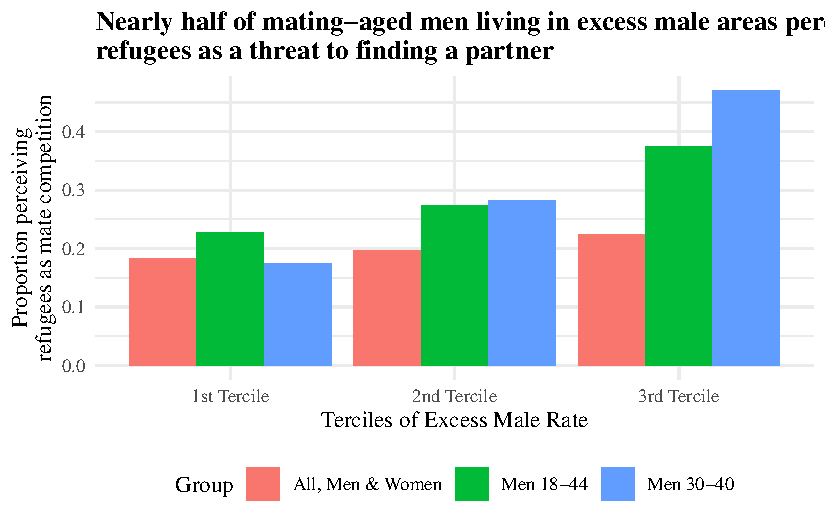
\includegraphics{paper_files/figure-pdf/fig-excess-1.pdf}

}

\caption{\label{fig-excess}Proportion of respondents who see refugees as
a mating threat by age group and tercile}

\end{figure}

\clearpage

\hypertarget{tbl-stmt}{}
\begin{table}
\caption{\label{tbl-stmt}Statements used for surveying respondents }\tabularnewline

\centering
\begin{tabular}{>{\raggedright\arraybackslash}p{7em}>{\raggedright\arraybackslash}p{35em}}
\toprule
Type & Statement\\
\midrule
\textbf{Only means} & When it comes to the refugee problem, violence is sometimes the only means that citizens have to get the attention of German politicians.\\
\textbf{Message} & Attacks against refugee homes are sometimes necessary to make it clear to politicians that we have a refugee problem.\\
\textbf{Justified} & Hostility against refugees is sometimes justified, even when it ends up in violence.\\
\textbf{Prevent} & Xenophobic acts of violence are defensible if they result in fewer refugees settling in town.\\
\textbf{Condemn} & Politicians should condemn attacks against refugees more forcefully. (For this statement, the results were reversed such that we are looking at respondents who Disagreed or Strongly Disagreed)\\
\bottomrule
\end{tabular}
\end{table}

\begin{figure}

{\centering 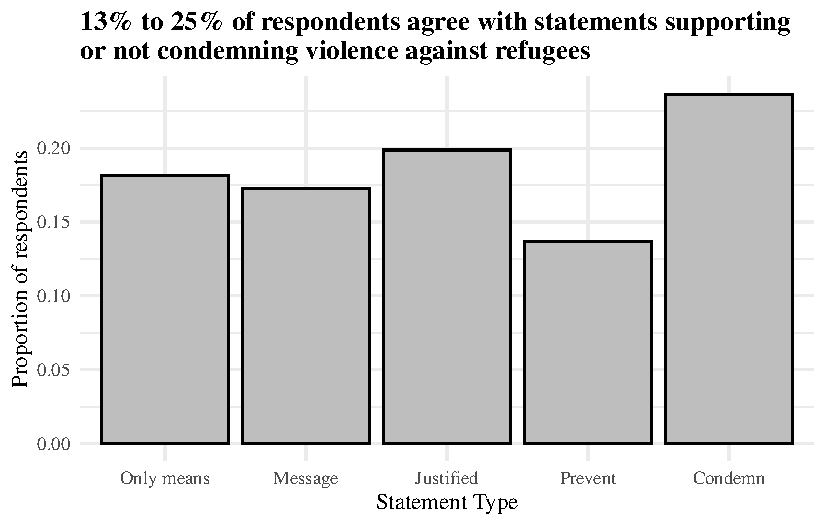
\includegraphics{paper_files/figure-pdf/fig-statements-1.pdf}

}

\caption{\label{fig-statements}Proportion of respondents who agree with
varying hate crime support statements}

\end{figure}

\renewcommand{\arraystretch}{1.5}

\begin{table}

\caption{\label{tbl-mate}Perceiving refugees as mate competition
predicts support for hate crime}\begin{minipage}[t]{\linewidth}
\subcaption{\label{tbl-mate-1}}

{\centering 

\centering
\resizebox{\linewidth}{!}{
\begin{tabular}{lccc}
\toprule
\textbf{} & \textbf{Model 1} & \textbf{Model 2} & \textbf{Model 3}\\
\midrule
Mate competition & 0.388954021258191 *** & 0.234463055537634 *** & 0.209649334128798 ***\\
 & (0.0145502521315924) & (0.0180328697220162) & (0.0182866642763472)\\
Job competition &  & 0.242797369618408 *** & 0.228877774924659 ***\\
 &  & (0.0181376984925587) & (0.0183883958329611)\\
Life satisfaction &  & -0.0333776515996499 * & -0.0308547572811113\\
\addlinespace
 &  & (0.0142614758807235) & (0.0157549163915511)\\
Sociodemographics &  &  & X\\
National attitudes toward refugees &  &  & \\
Local attitudes toward refugees &  &  & \\
Additional controls &  &  & \\
\addlinespace
N & 3019 & 3019 & 3008\\
R2 & 0.191496944608288 & 0.240300197343161 & 0.288264889594511\\
\bottomrule
\end{tabular}}

}

\end{minipage}%
\newline
\begin{minipage}[t]{\linewidth}
\subcaption{\label{tbl-mate-2}}

{\centering 

\centering
\resizebox{\linewidth}{!}{
\begin{tabular}{lccc}
\toprule
\textbf{} & \textbf{Model 4} & \textbf{Model 5} & \textbf{Model 6}\\
\midrule
Mate competition & 0.183273513474463 *** & 0.164099823558722 *** & 0.137626497064367 ***\\
 & (0.0171833389920075) & (0.0172882988473202) & (0.0167588355706287)\\
Job competition & 0.0749936478139196 *** & 0.0631275039256767 *** & 0.0542635065110621 **\\
 & (0.018940196237162) & (0.0190445311910028) & (0.0183521654226738)\\
Life satisfaction & -0.00777875013768452 & -0.00448858390914464 & -0.000128152048344066\\
\addlinespace
 & (0.0146927218423728) & (0.0146338266554448) & (0.0141114004380655)\\
Sociodemographics & X & X & X\\
National attitudes toward refugees & X & X & X\\
Local attitudes toward refugees &  & X & X\\
Additional controls &  &  & X\\
\addlinespace
N & 3008 & 3008 & 3008\\
R2 & 0.394249027379152 & 0.409657634382106 & 0.459150252350734\\
\bottomrule
\multicolumn{4}{l}{\rule{0pt}{1em}\textit{Note: }}\\
\multicolumn{4}{l}{\rule{0pt}{1em}All continuous predictors are mean-centered and scaled by 1 standard deviation.  *** p < 0.001;  ** p < 0.01;  * p < 0.05.}\\
\end{tabular}}

}

\end{minipage}%

\end{table}

\hypertarget{discussion}{%
\section{Discussion}\label{discussion}}

\hypertarget{findings}{%
\subsection{Findings}\label{findings}}

\hypertarget{implications}{%
\subsection{Implications}\label{implications}}

\hypertarget{ethical-implications}{%
\subsection{Ethical Implications}\label{ethical-implications}}

In their paper, Dancygier, Egami, Jamal, and Rischke examine the ethical
implication of using experimental methodologies to investigate their
research topic. By using descriptive data in the form of surveys they
are able to investigate the opinions of non-immigrant German males and
their perception of mate competition and its translation to anti-refugee
violence. By avoiding experimental trials, they were able to explore
their topic without provoking anti-refugee sentiment, which might have
been a possible outcome had trials been conducted (Dancygier et al.
2021). While conducting experimental trials on this topic of research is
considered unethical, surveys and questionnaires may have a tendency to
give respondents the impression that their opinions are commonly shared
or even accurate. By being presented with a platform to express their
perception of mate competition and if they agree that violence towards
refugees is the only way to garner the attention of German politicians,
respondents may feel that their opinions are incorrectly justified. This
then has the potential to translate to violence towards German refugees.

\hypertarget{accounting-for-bias}{%
\subsection{Accounting for Bias}\label{accounting-for-bias}}

Ethical implications and biases arise naturally when collecting
quantitative and qualitative data. In their paper, Dancygier, Egami,
Jamal, and Rischke use online survey platforms to assess if Germans
living in areas with greater populations of men who experience turmoil
in the mating market are more likely to perceive competition between
themselves and refugees, moreover, does this ideology predict hate crime
support (Dancygier et al. 2021). The authors attempted to address
ethical concerns and statistical biases by utilizing control groups and
replicating their study with different samples and polling firms.
However, one potential bias that is challenging to control for is the
presence of sampling bias (Dancygier et al. 2021). Sampling bias occurs
when participants in a study are not representative of the estimand or
the ideal population of interest. One method to control for this bias is
simple random sampling, where participants are chosen by chance. Meaning
that every individual in the population/ estimand has an equal chance of
being selected. However, in their study, they were unable to utilize
simple random sampling. Instead attempted to make their survey results
representative by conducting four waves of surveys meant to be
representative of age, gender and state/ geographical region
{[}Dancygier et al. (2021)\}. Despite their effort, their survey results
may not be entirely representative as individuals who have a strong
interest in the subject matter are more likely to participate, meaning
they do not reflect the views of all non-immigrant German males
(Dancygier et al. 2021).

\hypertarget{limitations}{%
\subsection{Limitations}\label{limitations}}

\hypertarget{future-research}{%
\subsection{Future Research}\label{future-research}}

\clearpage

\hypertarget{references}{%
\section*{References}\label{references}}
\addcontentsline{toc}{section}{References}

\hypertarget{refs}{}
\begin{CSLReferences}{1}{0}
\leavevmode\vadjust pre{\hypertarget{ref-government_of_canada_2022}{}}%
{``2022 Annual Report to Parliament on Immigration.''} 2022.
\emph{Government of Canada}, November.
\url{https://www.canada.ca/en/immigration-refugees-citizenship/corporate/publications-manuals/annual-report-parliament-immigration-2022.html}.

\leavevmode\vadjust pre{\hypertarget{ref-list}{}}%
Blair, Graeme, and Kosuke Imai. 2010. {``{list}: Statistical Methods for
the Item Count Technique and List Experiment.''} Available at The
Comprehensive R Archive Network (CRAN).
\url{https://CRAN.R-project.org/package=list}.

\leavevmode\vadjust pre{\hypertarget{ref-main_paper}{}}%
Dancygier, Rafaela, Naoki Egami, Amaney Jamal, and Ramona Rischke. 2021.
{``Hate Crimes and Gender Imbalances: Fears over Mate Competition and
Violence Against Refugees.''} \emph{American Journal of Political
Science} 66 (2): 501--15. \url{https://doi.org/10.1111/ajps.12595}.

\leavevmode\vadjust pre{\hypertarget{ref-readstata13}{}}%
Garbuszus, Jan Marvin, and Sebastian Jeworutzki. 2021.
\emph{Readstata13: Import 'Stata' Data Files}.
\url{https://CRAN.R-project.org/package=readstata13}.

\leavevmode\vadjust pre{\hypertarget{ref-huxtable}{}}%
Hugh-Jones, David. 2022. \emph{Huxtable: Easily Create and Style Tables
for LaTeX, HTML and Other Formats}.
\url{https://CRAN.R-project.org/package=huxtable}.

\leavevmode\vadjust pre{\hypertarget{ref-jtools}{}}%
Long, Jacob A. 2022. \emph{Jtools: Analysis and Presentation of Social
Scientific Data}. \url{https://cran.r-project.org/package=jtools}.

\leavevmode\vadjust pre{\hypertarget{ref-moreau_wang_2022}{}}%
Moreau, Gregory, and Jing Hui Wang. 2022. {``Police-Reported Hate Crime
in Canada, 2020.''} \emph{Government of Canada, Statistics Canada},
March.
\url{https://www150.statcan.gc.ca/n1/pub/85-002-x/2022001/article/00005-eng.htm}.

\leavevmode\vadjust pre{\hypertarget{ref-here}{}}%
Müller, Kirill. 2020. \emph{Here: A Simpler Way to Find Your Files}.
\url{https://CRAN.R-project.org/package=here}.

\leavevmode\vadjust pre{\hypertarget{ref-citeR}{}}%
R Core Team. 2020. \emph{R: A Language and Environment for Statistical
Computing}. Vienna, Austria: R Foundation for Statistical Computing.
\url{https://www.R-project.org/}.

\leavevmode\vadjust pre{\hypertarget{ref-pBrackets}{}}%
Schulz, Andreas. 2021. \emph{pBrackets: Plot Brackets}.
\url{https://CRAN.R-project.org/package=pBrackets}.

\leavevmode\vadjust pre{\hypertarget{ref-MASS}{}}%
Venables, W. N., and B. D. Ripley. 2002. \emph{Modern Applied Statistics
with s}. Fourth. New York: Springer.
\url{https://www.stats.ox.ac.uk/pub/MASS4/}.

\leavevmode\vadjust pre{\hypertarget{ref-tidyverse}{}}%
Wickham, Hadley, Mara Averick, Jennifer Bryan, Winston Chang, Lucy
D'Agostino McGowan, Romain François, Garrett Grolemund, et al. 2019.
{``Welcome to the {tidyverse}.''} \emph{Journal of Open Source Software}
4 (43): 1686. \url{https://doi.org/10.21105/joss.01686}.

\leavevmode\vadjust pre{\hypertarget{ref-dplyr}{}}%
Wickham, Hadley, Romain François, Lionel Henry, and Kirill Müller. 2022.
\emph{Dplyr: A Grammar of Data Manipulation}.
\url{https://CRAN.R-project.org/package=dplyr}.

\leavevmode\vadjust pre{\hypertarget{ref-readr}{}}%
Wickham, Hadley, Jim Hester, and Jennifer Bryan. 2023. \emph{Readr: Read
Rectangular Text Data}. \url{https://CRAN.R-project.org/package=readr}.

\leavevmode\vadjust pre{\hypertarget{ref-knitr}{}}%
Xie, Yihui. 2014. {``Knitr: A Comprehensive Tool for Reproducible
Research in {R}.''} In \emph{Implementing Reproducible Computational
Research}, edited by Victoria Stodden, Friedrich Leisch, and Roger D.
Peng. Chapman; Hall/CRC.

\leavevmode\vadjust pre{\hypertarget{ref-sandwich}{}}%
Zeileis, Achim. 2006. {``Object-Oriented Computation of Sandwich
Estimators.''} \emph{Journal of Statistical Software} 16 (9): 1--16.
\url{https://doi.org/10.18637/jss.v016.i09}.

\leavevmode\vadjust pre{\hypertarget{ref-lmtest}{}}%
Zeileis, Achim, and Torsten Hothorn. 2002. {``Diagnostic Checking in
Regression Relationships.''} \emph{R News} 2 (3): 7--10.
\url{https://CRAN.R-project.org/doc/Rnews/}.

\leavevmode\vadjust pre{\hypertarget{ref-kableExtra}{}}%
Zhu, Hao. 2021. \emph{kableExtra: Construct Complex Table with 'Kable'
and Pipe Syntax}. \url{https://CRAN.R-project.org/package=kableExtra}.

\end{CSLReferences}



\end{document}
